\documentclass{sig-alt-release2}
\usepackage{url}
\usepackage{color}
\usepackage{graphics,graphicx}

\usepackage{epsfig}
\usepackage{epstopdf}

\usepackage{colortbl}
\usepackage{multirow}
\usepackage{booktabs}
\usepackage{ifthen}  

\usepackage[table]{xcolor}
\usepackage{listings,multicol}
\usepackage{url}
\usepackage{cite}
\usepackage[numbers]{natbib}

\begin{document}
\newcommand{\todo}[1]{\textcolor{red}{#1}}
\def\newblock{\hskip .11em plus .33em minus .07em}

\conferenceinfo{DIM3} {2010, Glasgow, UK} 
\CopyrightYear{2010}
\clubpenalty=10000
\widowpenalty = 10000

\title{{Flat Organizer}}

\numberofauthors{1}
\author{
\alignauthor
Benjamin Behm\\
Daniel Tandberg Abrahamsen\\
Haakon S{\o}nsteby\\
	   \affaddr{Team Nordic}\\
      \affaddr{itech}\\
      \affaddr{2077473b, 2054832a, 2056007s}\\
             \email{\{ 2077473b, 2054832a, 2056007s\}@students.glasgow.ac.uk }
}
\maketitle

\begin{abstract}
Flat Organizer is a web application that helps people to manage tasks in households. It provides a simple interface, where users can keep a track of tasks that need to be done. The main page contains two different list: a continuous chores list, and a shopping list. A continuous chores list is meant to be for tasks that does not expire, but can be done regularly. A shopping list is for keeping list of items that should be bought to the household. In addition, Flat Organizer provides a simple view of what each member of the household has done and when. Each task will be scored based on how challenge it is to perform. Users' points will increase as they perform tasks.

\end{abstract}

\section{Aim of Application}
Most people lives in one a kind of household, it might be with their family, partner, roommates or perhaps some sort of student accommodation. While living in a household there are obligations among the residents that have to be fulfilled. Flat Organizer will make sure that each person in the household will contribute to the fellowship by both listing things that have to be done, and maybe even more important, shows a record of what everyone has completed in the last period of time.

\subsection{Functional Requirements}

We used so called MoSCoW technique to prioritize required functionalities. There are four different categories: 
\begin{itemize}
\item \textbf{M} = Must have
\item \textbf{S} = Should have
\item \textbf{C} = Could have
\item \textbf{W} = Would not have
\end{itemize}
	
\begin{center}
	\rowcolors{1}{gray}{white}
    \begin{tabular}{ | l | p{3.5cm} | l |}
    \hline
	 \textbf{ID}	& \textbf{Name} & \textbf{Priority} \\ \hline
    FR-1.1	& Show all flats a user is a member of & M \\ \hline
	FR-1.2	& Select a flat, that the user is member of & M \\ \hline
	FR-1.3	& Create a new flat, providing a flat name, description & M \\ \hline
	FR-1.4	& Invite members to flat	& M \\ \hline
	FR-1.5	& Allow invited members to join a flat	&	M \\ \hline
	FR-1.6	& Edit the name, description and members of a flat & S \\ \hline
	FR-1.7	& Delete a flat & S \\ \hline
	FR-1.8	& Allow users to leave a flat & S \\ \hline
	FR-2.1	& Show all tasks related to a flat & M \\ \hline
	FR-2.2	& Create a new task, by specifying name, description and category & M \\ \hline
	FR-2.3	& Select a task, and set a task as done	& M \\ \hline
	FR-2.4	& Delete a task	& S \\ \hline
	FR-3.1	& View high score by user & S \\ \hline
	FR-3.2	& See a user's recently completed tasks	& S \\ \hline
	Fr-4.1	& Create a new account, providing first name, last name, email, and 		password	& M \\ \hline
	Fr-4.2	& Log in with their credentials	& M \\ \hline
	Fr-4.3	& Log in with their Facebook/Gmail account	& W \\ \hline
	Fr-4.4	& Forgotten password functionality	& S \\
    \hline
    \end{tabular}
\end{center}

\subsection{Nonfunctional Requirements}
\begin{itemize}
\item Responsive UI, screen resolution down to 800x600 px must be supported
\item The application must work on the most common browsers: Google Chrome and Mozilla Firefox 
\item All data must be available in the data storage even though the user deletes it.
\item Security and authorization over entire application
\item All operations should be performed within a second, as after a couple seconds a user will start thinking that something is broken.
\item Any personal information should not be accessed by outsider.
\item Good usability.
\end{itemize}

\subsection{Assumptions}

The implemented application will be used on laptop or desktop as it is not designed for mobile using. Actually this application would be primarily used on mobile devices, but that would be implemented afterwards if the team continue to extend the application after delivery. 

\subsection{Design goals}

The overall design goals is allowing users to create and join flats, create and complete tasks and keep track of who did what in a flat. This should be accomplished by letting the user interact with an interface following the Keep It Short and Simple (KISS) guidelines. This is a functional, target driven application, so the number of disturbing elements should be minimized and the focus should rather be on letting the user do his/her's desired task in a simplistic, neat way. Less is more. 

\textbf{Constraints}
Time is one big constraint, but managing the time and estimating the tasks so that the scope of the application is appropriate may be even harder. None of the team members has any knowledge of Django or Python, so this is a new web development framework and programing language for all team members to become comfortable in. Some team members has a small amount of HTML, CSS and JavaScript experience, but this is very basic. When it comes to the three person team size, this is both an advantage and a disadvantage. Only three people makes the project easier to manage, communication flow is easier and every group member can be involved in all parts of the system. The disadvantage is that more people would generate more inputs on ideas, most likely have more knowledge and can produce more features to an application. //Just jibber the last sentence? 

Estimating the appropriate scope of the application is challenging. Especially when the web framework is new to every team member, giving no knowledge regarding the features it supports "out of the box". To try to overcome this problem priorities are used on every functionality implemented, so that core functionality is in place and more features can be implemented if time. The team realizes that the selected scope is ambitious, but feels that it it needs to be of this size in order to work as a complete, usable application.

\section{Client Interface}

\textbf{Wireframes}

\begin{enumerate}
\item Logo of the application that also works as a link back to the flat overview. 
\item Description of the flat, containing a picture, name of the flat, and the current members. The plus icon will show a small text field that is used to invite new members
\item Contains a list of the continuous tasks that needs to be done inside a flat. Every task has credits, a done button and a delete icon. 
\item Shopping list contains the items that only needs to be done once. Every item has a name, credits, a done button and a delete icon. 
\item The highscore list will show all the users, with their total points and last completed task, giving a quick and easy view of the score in the flat. 
\item The users name and profile picture is clickable and gives access to a dropdown menu, giving the options to sign out. 
\end{enumerate}

\begin{figure}[!ht]
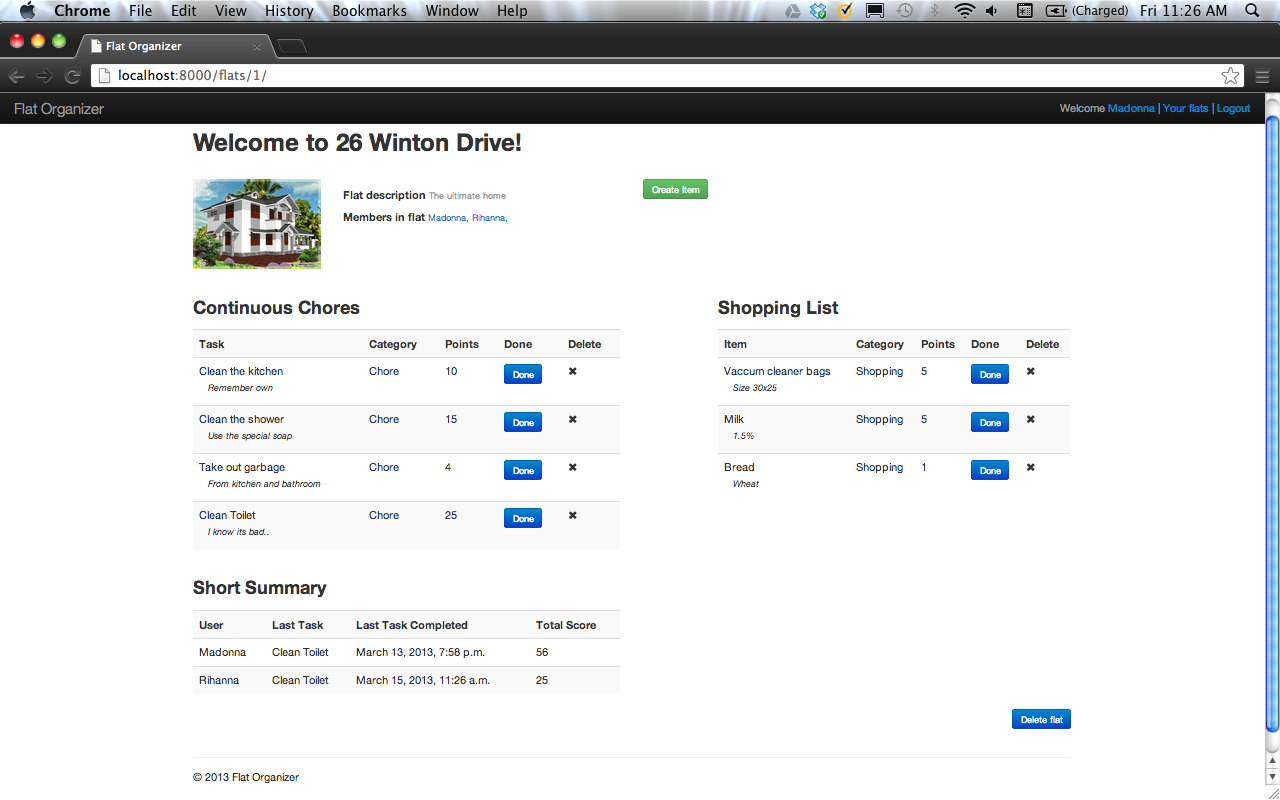
\includegraphics[scale=0.2]{tasks}
\caption{Main page}
\label{fig:mainpage}
\end{figure}	
	
//Insert Flat page CreateItem wireframe
\begin{enumerate}
\item By clicking on the upper right plus sign on either task list or shopping list a modal window will pop up, allowing the user to create a new item by filling in the appropriate values.
\end{enumerate}

//Insert Flats page wireframe
\begin{enumerate}
\item Logo of the application that also works as a link back to this view
\item A list of all the flats the user is currently a member of, giving the picture, name and other members. 
\item A list of flats the user has been invited to join. 
\item The new flat button will trigger a modal window to be displayed and the user can fill in the appropriate information.
\item The users name and profile picture is clickable and gives access to a dropdown menu, giving the options to sign out.
\end{enumerate}

\textbf{Use case descriptions}

\textbf{Use case}: Create a new shopping item.\\
\textbf{Summary}: User can create a new shopping item that appears in shopping list.\\
\textbf{Actors}: User \\
\textbf{Preconditions}: There is not this particular shopping list item. \\
\textbf{Goal of the primary user}: User wants to remember what (s)he needs to buy when in shop. \\
\textbf{Basic sequence}:
\begin{enumerate}
\item User selects the appropriate flat.
\item User clicks on the upper right plus sign in the shopping list area. 
\item User fills in a name, description, number of credits, and selects “Shopping list” from the drop down menu. 
\item User submits the item.
\item The item pops up in the shopping list.
\end{enumerate}
\textbf{Exceptions}:
\begin{itemize}
\item \textbf{Step 4}: User types wrong values on the form and get notification. Submit is not accepted.
\end{itemize}
\textbf{Postconditions}: New shopping list item appears on the shopping list. \\

\textbf{Use case}: Set shopping item as done. \\
\textbf{Summary}: After buying a item that has been on shopping list, a user want to set it done. \\
\textbf{Actor}: User \\
\textbf{Preconditions}: There is an item on shopping list. \\
\textbf{Goal of the primary user}: User wants to show that (s)he has participated in the work of a common flat and bought an item that was on the shopping list. \\
\textbf{Basic sequences}:
\begin{enumerate}
\item User selects the appropriate flat.
\item User finds the shopping item and clicks the “done” button
\item The item disappears from the shopping list.
\item The highscore table is updated with total score and the latest task.
\end{enumerate}
\textbf{Postconditions}: The shopping item has disappeared from the shopping list and a user has got points equivalent with the points of done task. \\

\textbf{Use case}: Create new flat and invite Justin Timberlake. \\
\textbf{Summary}: A user has just moved in a new flat and want to create a new flat. As Justin Timberlake moved in with her, she wants to send invite to him. \\
\textbf{Actor}: User and a secondary user \\
\textbf{Preconditions}: Both users have registered on the service.  \\
\textbf{Goal of the primary user}: User want to create a new flat, as she has just moved in a new flat. In addition, she want to invite her friends, so that they can easily divide common tasks in the flat community. \\
\textbf{Basic sequences}:
\begin{enumerate}
\item User clicks the "New flat" button.
\item User fills in name and description in the modal window.
\item User clicks the "Create" button.
\item A new flat appears on the Flats page.
\item User clicks on the invite link.
\item User fills in the email address of the other member.
\item User submits the invite.
\end{enumerate}
\textbf{Postconditions}: Invitation appears on the Flats page of the secondary user, and as he accept the invitation, his name will be shown on the Flat information of that flat and the User can also see that. \\

\subsection{Front-end technologies}

The technologies used to develop the front end is a combination of HTML5 and JavaScript, styled with the CSS toolkit Twitter Bootstrap \cite{x14}. The team used an external JavaScript library called jQuery \cite{x15} which simplified the client side scripting and provided easy access to new features. As for the discussion of implementing POST queries using Ajax, the team decided that Ajax is considered a luxury feature and will be implemented if time. All these technologies and extensions are well established with their own community and thorough documentation. There are other CSS toolkits out here, like blueprint \cite{x16}, HTML5BoilerPlate \cite{x17}, and Zurb \cite{x18}, but Bootstrap was chosen because of its popularity and community size. 

The achievement of using all these well established technologies and libraries is a set of predefined layout guidelines and elements allowing the team to easily make use of this instead of reinventing the wheel. This helped us to make Flat Organizer a neat, clean and intuitive application, where the users immediately finds themselves at home and can conduct their preferred task quick and easily.

\section{Application Architecture}

\subsubsection{N-Tier architecture}
FlatOrganizer consists of a 3-Tier layered architecture. The separation of concerns (the three independent layers) makes it easy to develop and manage. In addition Django is based on the MVC (Model-View-Controller pattern) even though one might say that MTV (Model-Template-View) is more accurate if acronyms are important \cite{django1}. This way of both implementing the application and the mindset this structure forces, ensures separation of concerns.

The front end (presentation layer) which is presented to the client is loaded after http requests. The clients are usually web browsers, and the requests are mostly based on URLs and form submits. The front end technologies in FlatOrganizer are HTML, CSS, JavaScript and jQuery.

The application layer in FlatOrganizer is implemented with Django, a Python Web Framework. It is the logical part of the application which handles client requests, maps URLs, performs calculations, and retrieves data from the data layer.

The data layer, the database, is a SQLite database that is a lightweight database management system and easily used with Django applications.

\begin{figure}[!ht]
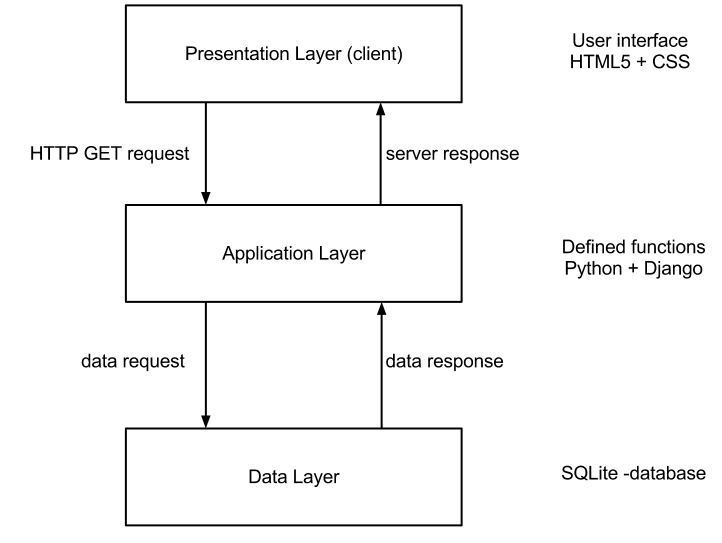
\includegraphics[scale=0.3]{3tier}
\caption{ 3-Tier Architecture Diagram}
\label{fig:3tier}
\end{figure}


\subsubsection{ER model}
In Figure~\ref{fig:er} below shows the ER-model, and the database is implemented as a relational database. For the implementation we used Django's SQLite support. By creating classes and relations in the model (models.py) we are able to let Django handle the requests (e.g. INSERT, DELETE, SELECT statements) with its ORM (Object Relational Mapper) (Managers).

\begin{figure}[!ht]
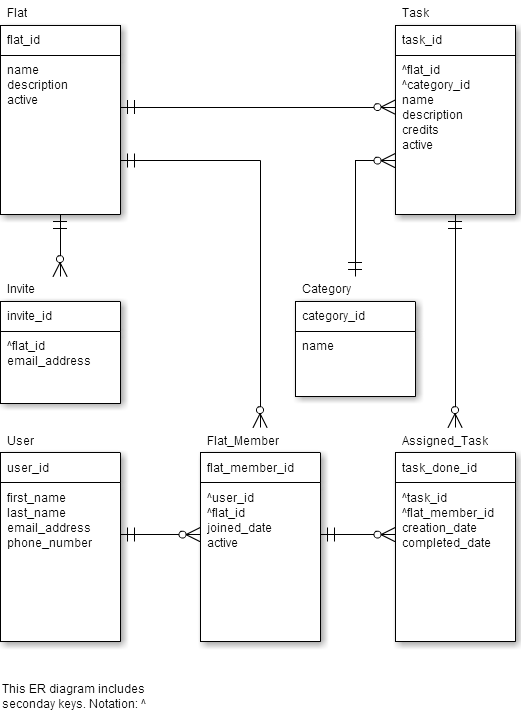
\includegraphics[scale=0.3]{er}
\caption{ ER diagram}
\label{fig:er}
\end{figure}

\textbf{Web Framework: Django}
Django suits our project perfectly and is a recognized and easy to use Python web framework. However there are many web frameworks out there. Other frameworks are for example Flask (Python) \citenum{x1}, Pylon (Python) \cite{x2}, Grok (Python) \cite{x3} and TurboGears (Python) \cite{x4}, JSF (Java) \cite{x5}, Apache Struts (Java) \cite{x6}, CakePHP (PHP) \cite{x7}, ASP (.NET) \cite{x8} and maybe the strongest competitor Ruby on Rails (Rails) \cite{x9} \cite{x19}. They all support N-tier architecture with focus on web development.
 
Web Application Frameworks focus on building web applications, and the main advantages are functionality such as session management and user authentication, data persistence and template systems \cite{x10}.

Even though Web Application Framework has a lot of advantages there are some disadvantages that must be considered before selecting a framework. These disadvantages could be performance issues, one might need education in a specific language and framework to be able to develop efficiently, customization of functions and functionality might be hard, and if bugs and security issues are discovered, all applications that use the framework could be affected. \cite{x11}

\section{Message Parsing}

\textbf{HTTP} (Web Server Request Format)
The HTTP request is sent with either of the following methods:
\begin{itemize}
\item POST requests for form submissions
\item GET request for standards HTTP request
\end{itemize}
HTTP (Hypertext Transfer Protocol) is the standard World-Wide-Web protocol for sending messages.

An example message could look like this

\begin{figure}[!ht]
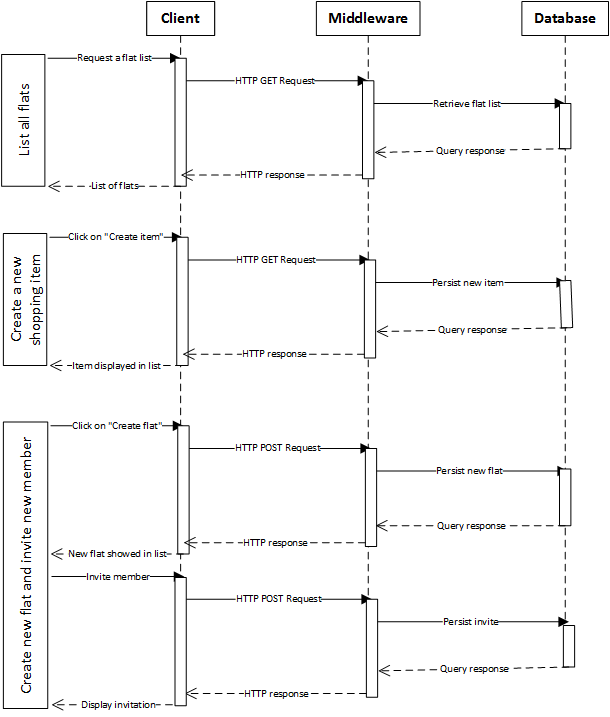
\includegraphics[scale=0.55]{sequencediagrams}
\caption{Sequence diagrams}
\label{fig:sequence}
\end{figure}
 
\textbf{Database Request Format}
The connection between the database and the application is SQLite format. These transactions/requests are handled by Django.

These messages are formatted as SQL statements such as: 
\begin{verbatim} SELECT * FROM flats_flat \end{verbatim}



\section{Implementation Notes}

Views
FlatOrganizer has only one view.py file, but implements many functions (redirected through the URL dispatcher). The following functions exist:

\begin{itemize}
\item def index(request)
\item def flat(request, flatid=None)
\item def profile(request, flatid=None, username=None)
\end{itemize}
Depending on a flat id, this will redirect either to the personal profile (no flat id argument), or to the users profile within one flat.
\begin{itemize}
\item def register(request)
\item def user{\_}logout(request)
\item def user{\_}login(request)
\end{itemize}
URL Mapping Schema
The following code snippet is the main URL patterns in FlatOrganizer. Every pattern redirects the client to the correct method (second argument) in views.py.

lstset{language=HTML} 

\begin{lstlisting}[language=HTML, numbers=left, linewidth=8.5cm, breaklines=true, breakautoindent=true]
urlpatterns = patterns('',
	url(r'^$', views.index, name='index'),
	url(r'^register/$', views.register, name='register'),
	url(r'^login/$', views.user_login, name='login'),
	url(r'^logout/$', views.user_logout, name='logout'),
    url(r'^(?P<flatid>\d+)/(?P<username>\w+)/$',views.profile, name='flatuser'),
	url(r'^profile/$', views.profile, name='profile'),
   	url(r'^(?P<flatid>\d+)/$', views.flat, name='flat'),
\end{lstlisting}



The code snippet above results in the following URLs (after: http://servername/flats/:
index, register, login, logout, <flatid>, <flatid>/<username>, profile.

External Services
We did not use any external services (only serviced within the Django environment).

To be able to send email, a SMTP server was needed. During the demonstration we used Gmails SMTP server and one personal Gmail account to make this work. However we needed only to add the account settings to settings.py and from there, Django packages handled the rest.


\textbf{Functionality Checklist}
\begin{itemize}
\item List all flats a user is a member of
\item Create a new flat
\item Invite members to flat by email
\item Allow invited members to join a flat 
\item Edit the name, description and members of a flat
\item Allow users to leave flat
\item Delete a flat
\item Show all tasks related to a flat
\item Create a new task inside a flat
\item Select a task, and set a task as done
\item Delete a task
\item View overall high score in a flat
\item See a user’s recently completed tasks
\item Inspect roommates{’} profiles
\item Edit personal informations
\item Create a new account, providing first name, last name, email, and password
\item Log in with their credentials
\end{itemize}

\textbf{Known Issues}
There are no known issues (bugs), but take a look at the improvement section for functionality that could and perhaps should be improved.

\textbf{Technologies}

\begin{center}
	\rowcolors{1}{gray}{white}
    \begin{tabular}{ | p{1.7cm} | p{3.5cm} | p{2cm} |}
    \hline
	 \textbf{Technology} & \textbf{Description} & \textbf{Category} \\ \hline
	
	Python & Object oriented and dynamic programming language. &	Programming Language \\ \hline
	Django & High-level Python Web framework based.&	Web Framework \\ \hline
	HTML & Creates web pages.	&Markup Language \\ \hline
	CSS	& Describes the presentation semantics of the markup language.&	Style Sheet Language \\ \hline
	JavaScript & Interpreted programming language. Used as a dynamic script language to alter DOM. & Programming Language \\ \hline
	jQuery & Makes HTML document traversal and manipulation easier. Multi and cross browser support. &	JavaScript Library \\ \hline
	Bootstrap & A collection of tools for creating and styling web pages. & CSS, JavaScript extension \\
	
    \hline
    \end{tabular}
\end{center}

Even though Ajax is not implemented, Flat Organizer would benefit of it. The implementation of Ajax was planned but with a lower priority (it was considered a luxury feature and was given a lower priority). Ajax (Asynchronous JavaScript and XML) consists of JavaScript and the object XMLHttpRequest, and is actually not a separate technology. Even though the messages originally were sent as XML, the JSON format is more and more used. Ajax is often used in web development at the client side to create asynchronous messages (messages that are sent in background) to the application layer. These messages are sent to the server side without the need of refreshing a page. JavaScript or jQuery is then often used for altering the DOM with new data (the response). A good tool for implementing Ajax within the Django Framework is Dajax [1].

\section{Reflective Summary}

\textbf{What have we learnt through the process of development?}

We learned a lot about different web development technologies, such as HTML5, CSS, JavaScript, Python, and Django. These were quite a new area of study for most of us. In addition, none of us had never used Python or Django before. This course was extremely beneficial for us and gave us readiness to develop web application using previously mentioned techniques. We are sure that we will use Python/Django combination in future, as it provide a simple and logical way to implement web applications. 

This project increased our understanding of web applications in general. Now we understand much more better how the information flows in a web application, and what is the overall structure of it. We had heard that there is some http request and responses between client and server, but now we saw how those are actually happening. Furthermore, during the development process our understanding of how different technologies and protocols presented on lectures take part in different phases increased a lot.

We also used Git for version control management. Using Git reminded us how important it is to keep track of changes. As something went broken, it was easy to return to previous commit and check where the broken code was. In addition, two of us had not used Git for a while, so it was useful to recall how to use it, as it is widely used in software industry nowadays. 

\textbf{How did the frameworks help progress?}

As we had designed the layout beforehand, it was easy to follow those frameworks during the development process. Even though the layout changed from original drafts, those helped to understand what needed to be done as they concretized the view of the application. In this reason, it is really beneficial to draw some sort of drafts of the application as these help to imagine the entirety and estimate the progress.

\textbf{Problems}

We did not encountered major problems during the development process. We did not have previous experience with Python and Django, so every now and then some one got stuck with technical problem, for example how to make something work. Usually these were overcame fast with the support of other team members.

During the first weeks it was quite hard to follow what other team members were doing, and what should be done next. It helped a lot as we started using Github{’}s issue tracker, where we listed all tasks and issues that needed to be done, and from where we saw which tasks were already started or done, and who was responsible with what.

\textbf{Major achievements}
 
The user interference is simple and intuitive. It is easily used and does not need time to learn how to use the most important functionalities. This is confirmed by the evaluation panel at the demo. We got a lot of good feedback from industry visitors. They especially praised following aspects:
\begin{itemize}
\item Neat user interface
\item Complete system
\item Responsiveness
\item Addressing real world situation
\end{itemize}
We can agree all of previous comments, and we are fairly proud of the result we got during the course.

\section{Summary and Future Work}

\textbf{Summary of application and its current state}

The application provides a simple interface to manage tasks of different flats. As a user can live in several flat (or apartment), (s)he might want to divide daily tasks efficiently with other roommates. The application is destined for that purposes. User can maintain two different list: a list of continuous chores and a shopping list. Former is meant for tasks that are running all the time and these stays on the list even if it is set done. Latter can be used to list items that need to be bought irregularly and are removed from the list as they are purchased.

The application is ready and functional, and it could be used in in real life. It has quite limited amount of functionalities, but it still contains all core functionalities that are needed to use it for task management.

\textbf{Limitations}

Current name of application and an user interface can make it look like it can be only used by people who lives in flats, like students. Of course the application can be used, for example, by families that lives in their own detached houses and want to keep track of tasks that every family member should do.

Security aspect can be seen as a limitation, as currently user’s password can be phished, as it is sent as a plain text using POST method. It should be salted all the time in order to increase security.

\textbf{Plans for future development}

There would be a clear market for this kind of application. We should not only focus on people living in flats, as this application could also be used in regular families. There are a huge amount of households that are struggling with coordinating daily tasks for each family members. Using Flat Organizer application, parents could easily inspect what their children have done and when. Parents could insist them to do some specific tasks in order to get a reward, which could be anything between playing PS3 and getting money for a movie night. This could be supported by implementing a functionality that allows users to take a picture before and after the task and attach these onto the task. This would make easier to follow that tasks are really done.

There are a lot of other functionalities that could be implemented in order to increase the value for users and improve the user experience. The application should be provided as a mobile application as this kind of applications would be primary used on mobile devices instead of computers. In this reason, we should develop a mobile application, which simplifies both task logging process and viewing new tasks. It should also contain a notification functionality, so that if a user is in a shop, (s)he would be notified when the shopping list is edited.

Currently a user needs to write every single task again and again, so instead of this there could be shortcut icons for most common tasks, so that a user could just click them to create new tasks. 

There are some issues relating to technology that should be fixed if the application is going to be published. Currently user password is sent as a plain text as user log in. This should absolutely be fixed. In addition, we could change the way how pages are refreshed after a form is sent. We could use AJAX in form submissions, which would also make possible to implement messages that are shown to users as they do something, for example, set task done.

In addition of previously mentioned implementation possibilities, we should put effort to implement following issues as those are usually required functionalities:

User can add a profile picture in registration, but cannot change it afterward.
There is a fixed flat picture, that cannot be changed.
Registration does not validate the user’s email. If other user has a same email, new user will get same invitations.
User cannot change a password, or get a new one if old is forgotten.
User cannot filter done tasks, so the list would grow very long as time elapses.
List all tasks a user has done in each of his/her flats.

\textbf{Another nice-to-have functionalities could be}:
\begin{itemize}
\item Trade in points: User can trade an amount of points to get something.
\item Find flats: User could be able to find flats.
\item Compare flatmates: Users could be able to compare each other.
\item Badges: Users get badges as they have done some tasks or got enough points.
\item Facebook connection: Send invitations and notifications via Facebook.
\item Money spend in addition to credits: Show how much money each has spend.
\item Timeout on tasks: Task could be set to expire on a specific day.
\end{itemize}
But that will set a constraint. If you have a party, and someone just washed the toilet - will noe get credit/points for doing that the next day when needed..

\textbf{Work distribution}

Benjamin: Login, user registration, front page
Daniel:
Haakon:

\section{Acknowledgements}

We want to thank the lecturer for inspiring lectures and giving good advices during labs.
We want to thank industrial visitors, who gave us valuable feedback during a demo session how to improve the application.

\bibliographystyle{abbrv}
\bibliography{sig-proc}

\end{document}